%\chapter{Часть третья. Объектно-ориетированное программирование на С++ с использованием \Sys{Qt} SDK}

\chapter{Знакомство с \Sys{Qt}. Подготовка к работе}
\section[Знакомство с \Sys{Qt}. Обзор истории]{Знакомство с \Sys{Qt}. Обзор истории}
Кроссплатформенный инструментарий разработки \Sys{Qt} появился впервые в 1995 году благодаря своим разработчикам
Хаарварду Норду и Айрику Чеймб-Ингу. С самого начала создавался как программный каркас, позволяющий 
создавать кроссплатформенные программы с графическим интерфейсом. Первая версия \Sys{Qt} вышла 
24 сентября 1995. Программы, разработанные с \Sys{Qt}, работали как под управлением операционных 
систем семейства \EN{Microsoft Windows\texttrademark} так и под управлением \EN{Unix}-подобных систем.

За годы разработки возможности \Sys{Qt} значительно выросли. Работа с сетью, базами данных, графикой,
мультимедиа, Интернет и другие расширения превратили его в универсальный инструментарий для создания программ. 
\Sys{Qt} превратился в полноценный и мощный инструмент разработки, который значительно превзошел свои первоначальные
возможности.

В июне 1999 года вышла вторая версия --- \Sys{Qt} 2.0. А в 2000 году состоялся выпуск версии для встраиваемых
систем, который назывался \Sys{Qt Embedded}. Версия \Sys{Qt} 3.0 --- 2001 год --- работала в ОС семейства 
\EN{Windows\texttrademark} и многих \EN{Unix}-подобных ОС, таких как \EN{MacOS}, \EN{xBSD}, в различных 
вариантах \EN{Linux} для персональных компьютеров и встраиваемых
систем. Он имел 42 дополнительных класса, объем вырос до более чем 500 000 строк кода. Летом 2005 года состоялся выпуск
\Sys{Qt} 4.0, который включал в совокупности около 500 классов и имел огромное количество существенных улучшений. Вместе с
выпуском \Sys{Qt} 4.5 вышло и специализированная интегрированная
среда разработки \Sys{QtCreator}.

В декабре 2012 состоялся официальный выпуск \Sys{Qt5}. Эта версия кроссплатформенного средства разработки
совместима с \Sys{Qt4}. Перенос кода с \Sys{Qt4} на \Sys{Qt5} не требует много усилий. В то же время, 
\Sys{Qt5} отличается рядом особенностей,
улучшений и большим количеством новых возможностей.

Современное программное обеспечение достаточно сложное и должно соответствовать многим требованиям. 
Кроме пользовательских требований, налагаемых на удобство и возможности программного продукта, есть 
и другие требования, касающиеся разработки программного обеспечения. Большую роль здесь играют средства, 
которыми программист пользуется в
процессе своей работы. Во многих случаях бывает удобно владеть инструментарием, который имеет достаточно широкую
область применения и может служить для решения большого количества задач разного масштаба: от построения небольших
программ для создания мощных программных пакетов. Также часто возникает вопрос о поддержке нескольких программных
платформ, ведь, ориентируясь только на одну платформу, можно потерять большое количество потенциальных
пользователей.  

Инструментарий разработки \Sys{Qt} используют для создания \index{Кроссплатформенная
программа}\emph{кроссплатформенных программ}. Здесь под этим утверждением мы
подразумеваем программы, исходный текст которых  можно скомпилировать на разных
\index{Программная платформа}программных платформах (различные разновидности \EN{Linux},
\EN{Windows}, \EN{MacOS} и т.д.) \emph{практически без изменений или с незначительными изменениями}.
Кроме того \Sys{Qt} используют и для разработки программ, имеющих характерный
(<<родной>>, native) для программного окружения или даже собственный
стилизованный интерфейс. Все это благодаря открытому свободному программному коду, удобному и 
логическому API и широким возможностям применения.

\Sys{Qt} расширяет возможности программиста с помощью набора макросов, метаинформации и сигнально-слотовых
соединений, но использует при этом лишь средства языка \Sys{C++} и является совместимым со всеми распространенными
современными его компиляторами. 

Наряду с традиционным для предыдущих версий \Sys{Qt} способом создания пользовательских интерфейсов, основанный
на \index{Виджеты}\emph{виджетах} --- визуальных элементах интерфейса
(кнопки, флажки, выпадающие списки, поля ввода, слайдеры и т.д.), \Sys{Qt5} ставит большой акцент на использовании технологии
QtQuick. В \Sys{Qt5} некоторые нововведения коснулись и синтаксиса для создания сигнально-слотовых соединений.

Программный код, зависящий от оконной системы в \Sys{Qt5}, был отделен и реорганизован в отдельные библиотеки
расширения, что позволило упростить перенос \Sys{Qt} на новые платформы и адаптации для поддержки других оконных систем.
Благодаря QPA (\Sys{Qt} \EN{Platform Abstraction}) в \Sys{Qt5} реализована поддержка многих платформ для мобильных устройств.

Несмотря на эти изменения и усовершенствования, большинство программного кода созданного для \Sys{Qt4}
совместимо с \Sys{Qt5} и компилируется с новой версией почти без изменений. Почти весь материал 
следующих разделов и примеры
подходят для изучения как \Sys{Qt4}, так и \Sys{Qt5}. Большая часть изменений в \Sys{Qt5} касается 
разделения на модули. 

\subsection{Основные составляющие \Sys{Qt}}
Рассмотрим основные составляющие кроссплатформенного средства разработки Qt: модули и инструменты.

На рис.~\ref{ch11:refDrawing0} изображены основные составляющие \Sys{Qt}. Модули и инструменты
доступны для разработки под целевые (\EN{Reference}) и другие (\EN{Other}) платформы. 
Средства \Sys{Qt} разделены по назначению на
отдельные части --- модули. Каждый из модулей выполнен в виде отдельной библиотеки. Разработчик имеет возможность выбрать
модули, которые он использует в программе. Модули имеют взаимозависимости: одни модули используют возможности, которые
предоставляют другие. Основу составляют \index{Модули Qt!основные (\EN{Essentials})}основные (\EN{Essentials}) модули:

\begin{figure}[htb]
\begin{center}
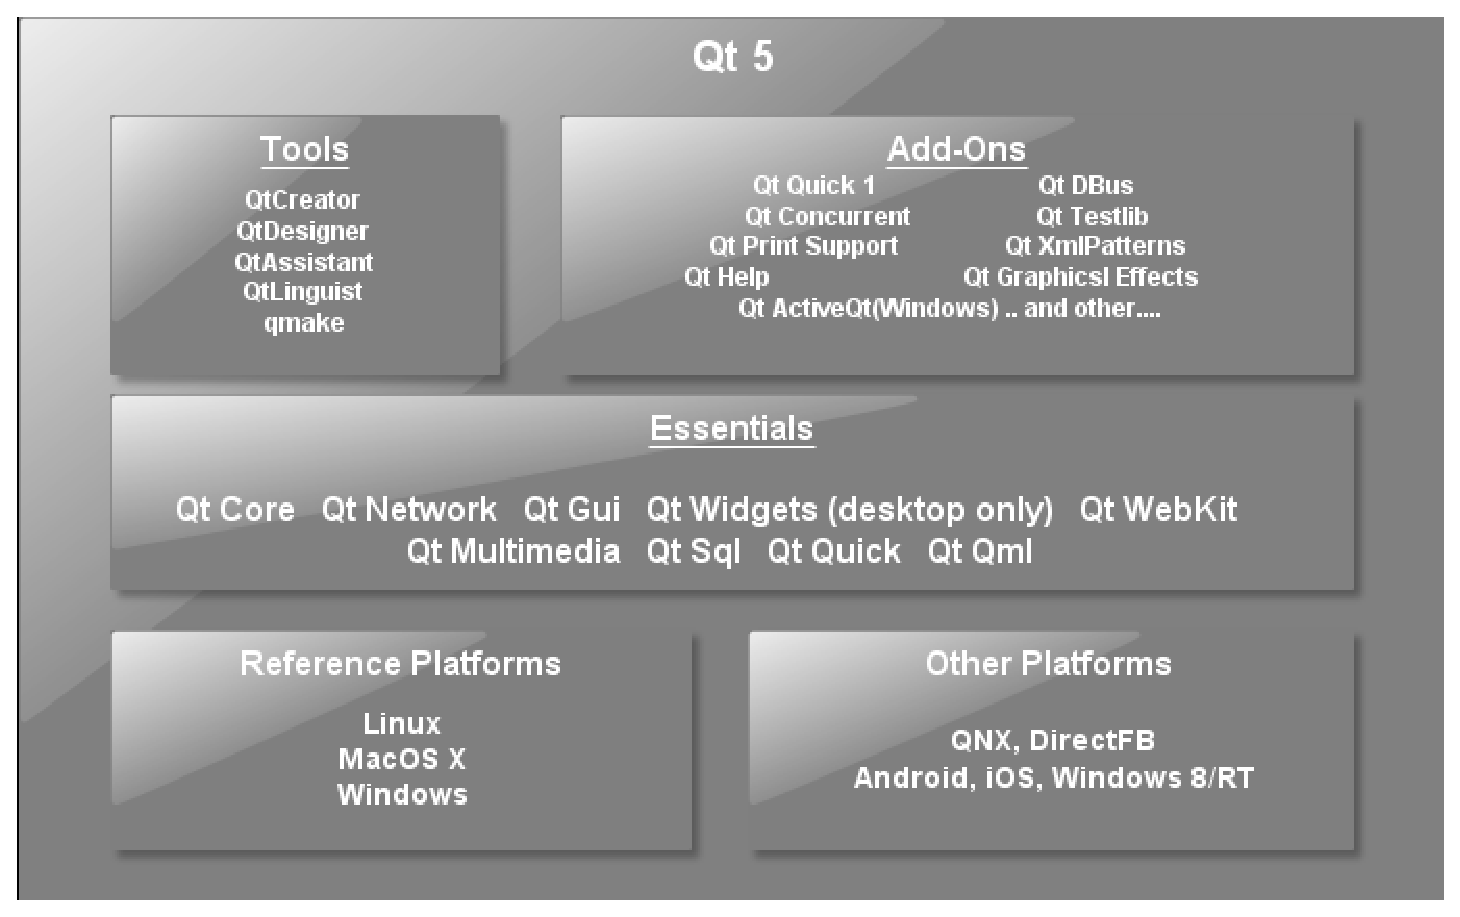
\includegraphics[width=0.7\textwidth]{img/ris_11_1}
\caption[Состав \Sys{Qt5}]{Состав \Sys{Qt5}}
\label{ch11:refDrawing0}
\end{center}
\end{figure}

\begin{itemize}
\item \Sys{Qt Core} --- основной модуль, который содержит все базовые средства \Sys{Qt}. На его основе
построены все другие модули. Каждая программа созданная с использованием \Sys{Qt}, использует
этот модуль;
\item \Sys{Qt Network} --- модуль для работы с сетевыми средствами;
\item \Sys{Qt Gui} --- модуль поддержки графического вывода на экран. В \Sys{Qt4} он также содержит содержит
набор виджетов для создания графического интерфейса пользователя. В \Sys{Qt5} виджеты вынесены в отдельный модуль;
\item \Sys{Qt Widgets} --- модуль, который содержит набор виджетов для создания графического интерфейса
пользователя (\Sys{Qt5})
\item \Sys{Qt WebKit} --- средства работы с Веб;
\item \Sys{Qt WebKit Widgets} --- виджеты для работы с Веб (\Sys{Qt5});
\item \Sys{Qt Multimedia} --- средства работы с мультимедийными устройствами и файлами;
\item \Sys{Qt Multimedia Widgets} --- виджеты для работы с мультимедийными устройствами и файлами (\Sys{Qt5});
\item \Sys{Qt Sql} --- средства работы с базами данных;
\item \Sys{Qt Qml} --- поддержка декларативной языка QML для разработки динамических визуальных
интерфейсов (\Sys{Qt5});
\item \Sys{Qt Quick} --- поддержка создания динамических визуальных интерфейсов (\Sys{Qt5});
\item \Sys{Qt Quick Controls} --- использование технологии QtQuick для создания традиционного для рабочих
столов графического интерфейса (\Sys{Qt5});
\item \Sys{Qt Quick Layouts} --- компоновка для элементов QtQuick (\Sys{Qt5}).
\end{itemize}

Существует также много \index{Модули Qt!дополнительные (Add-On)}дополнительных (Add-On) модулей. 
Стоит заметить, что разделение на основные и дополнительные
модули характерно \Sys{Qt5} в отличие от предыдущих версий. Названия некоторых модулей в \Sys{Qt5} по сравнению с \Sys{Qt4}
были изменены, а некоторые средства были вынесены в
отдельные или перенесены в другие модули. Эти изменения необходимо учитывать при переносе программ, которые были
разработаны с использованием \Sys{Qt4}. Почти все примеры, которые мы будем рассматривать, работают как с \Sys{Qt4} 
так и \Sys{Qt5}. В случаях, когда это существенно, мы будем указывать на отличия.

Кроме модулей, в состав инструментария входят инструменты разработки, исходные тексты \Sys{Qt}, примеры программ
и документация.

\section[Лицензирование \Sys{Qt} ]{Лицензирование \Sys{Qt}}
\Sys{Qt} распространяется по условиям трех различных лицензий: GNU GPL v3, GNU LGPL v3 и по коммерческой
лицензии компании \EN{Digia}. Здесь мы лишь кратко осмотрим основные положения этих лицензий и что это означает для
программ, которые используют соответственно лицензированный \Sys{Qt}.

\subsection[GPL]{GPL}
Программа должна быть открыта, свободно распространяться, исходные тексты программы и все изменения в
исходных текстов \Sys{Qt} должны пребывать в свободном доступе.

\subsection[LGPL]{LGPL}
Исходные тексты программы могут быть как открытыми так и закрытыми. В случае, если программа является
закрытой и планируется коммерческое использование программы --- \Sys{Qt} должен связываться с программой в виде
динамических библиотек. Конечно, в этом случае нельзя вставлять и использовать любые
исходные тексты \Sys{Qt} в программе. Также любые изменения в исходных текстах \Sys{Qt} должны быть 
пребывать в свободном доступе.

\subsection[Commercial]{Commercial}
В случае коммерческой лицензии, кроме возможности закрывать, модифицировать любым образом текст программы,
модифицировать или закрывать изменения в коде \Sys{Qt} и произвольно выбирать лицензию и способ распространения программы,
предоставляется также поддержка и консультации по использованию \Sys{Qt}.

\section[Справка и ресурсы]{Справка и ресурсы}
Важнейшей помощницей при разработке с использованием \Sys{Qt} является интегрированная справка. Документация \Sys{Qt}
удивительно удобна в использовании и создана для быстрого поиска среди богатого инструментария \Sys{Qt}. Она содержит не
только описания классов, входящих в состав модулей, но и краткие примеры использования методов и классов, полные тексты
демонстрационных программ, освещающих возможности \Sys{Qt}. Также здесь можно найти несколько пошаговых инструкций для
начинающих и статьи, посвященные описанию и
объяснению механизмов работы и различных аспектов использования инструментария.

Для просмотра интегрированной справки можно воспользоваться как средой \Sys{Qt Creator}, так и специальной
отдельной программой, которая называется \index{Инструменты Qt!\Sys{Qt Assistant}}\Sys{Qt Assistant}
и является частью инструментария \Sys{Qt}.

Для  вызова встроенной справки вы можете воспользоваться одним из следующих способов:

\begin{itemize}
\item перейдите в режим справки среды \Sys{Qt Creator} --- \Sys{Help} (комбинация клавиш \Sys{Ctr+7});
\item установите курсор на название класса или метода и нажмите \Sys{F1} --- среда выполнит поиск и откроет
соответствующий раздел справки в боковой панели.
\end{itemize}
В режиме справки или в случае использования \Sys{Qt Assistant} слева от окна документации расположена панель,
которая может переключаться в несколько различных режимов: Закладки (\EN{Bookmarks}),
Содержание (\EN{Contents}), Указатель (\EN{Index}) и Поиск (\EN{Search}). Режим панели определяется
выпадающим списком сверху. Особенно удобно пользоваться режимом Указатель (\EN{Index}) при работе: 
как только пользователь
вводит начало названия класса, метода или статьи, в справке выполняется поиск и отображение совпадений.
Это особенно пригодится для быстрой навигации и поиска в справке.

Следует помнить, что эта книга, как и любая другая, не может быть исчерпывающим обзором \Sys{Qt}, поэтому
дальнейшая работа с ней будет требовать параллельного исследования документации. Вот несколько советов:

\begin{itemize}
\item не пытайтесь запомнить все названия методов, классов и т. п. Сконцентрируйтесь на осмотре
возможностей, основных концепциях и практике. Используйте справку для быстрого поиска и восстановления в памяти тех или
иных деталей использования инструментов \Sys{Qt};
\item обратите внимание на большое количество примеров. Рассматривайте примеры параллельно с рассмотрением
материала в книге;
\item попробуйте сразу же находить классы и методы из следующих глав книги в справке и исследовать их, как
только вы начинаете их изучение. Для этого особенно
пригодится быстрая навигация и поиска в справке.
\end{itemize}
В сети Интернет существует большое количество ресурсов, статей, учебных видео посвященных \Sys{Qt}. Вот
важнейшие из них:

\begin{itemize}
\item \Sys{Qt Project} ({\small\url{http://qt-project.org/}}) --- главный сайт свободного инcтрументария разработки
\Sys{Qt};
\item \Sys{Qt Digia} ({\small\url{http://qt.digia.com/}}) --- официальный сайт коммерческой версии Qt;
\item \Sys{Planet Qt} ({\small\url{http://planet.qt-project.org/}}) --- сайт, который собрал десятки блогов посвященных
\Sys{Qt};
\item \Sys{Qt Centre} ({\small\url{http://www.qtcentre.org/}}) --- форум посвященный
вопросам разработки;
\item \Sys{Qt-Apps.org} ({\small\url{http://qt-apps.org/}}) --- сайт посвященный
открытому программному обеспечению созданному с использованием \Sys{Qt}.
\end{itemize}

\section[Обзор настроек среды \Sys{Qt Creator}]{Обзор настроек среды \Sys{Qt Creator}}
Для разработки программ с использованием библиотеки \Sys{Qt} была создана интегрированная среда разработки
\index{Инструменты Qt!\Sys{Qt Creator}}\Sys{Qt Creator}. Ее первая версия была представлена
одновременно с официальным выпуском \Sys{Qt} 4.5.0. Это полноценная кроссплатформенная
среда для создания новых проектов и работы с ними.

Мы рассмотрим работу со средой \Sys{Qt} Creator версии 2.8.0, которая позволяет управлять целым рядом этапов
разработки программы такими как: управление сеансами и проектами, редактирование и создание программного кода,
конструирование пользовательского интерфейса программы, анализ быстродействия, анализ использования ресурсов, отладка,
построение проекта, запуск программы.

Одно из первых действий, которое необходимо выполнить разработчику перед началом работы с \Sys{Qt Creator} --- это
настроить среду таким образом, чтобы с ней было удобно работать. Конечно, \Sys{Qt Creator}
имеет стандартные настройки, которые уже достаточно удобны для работы. Несмотря на это, мы хотели бы обратить ваше
внимание на некоторые настройки, которые особенно полезны в работе. Среди большого количества настроек мы рассмотрим
лишь наиболее важные для работы, а именно настройки компиляции и настройки редактора кода. Для доступа к диалогу
настройки используем главное меню (пункт \Sys{Tools}-> \Sys{Options...}, см. рис.~\ref{ch11:refDrawing1}).

Сначала коснемся настроек компиляции. Для управления настройками, относящимися к построению проекта, 
\Sys{Qt Creator} использует понятие комплекта (\EN{Kit}). \index{Комплект (Kit)}Комплект (\EN{Kit}) --- это конфигурация, 
которую составляют версия \Sys{Qt}, компилятор и еще
некоторые дополнительные настройки. Таким образом, QtCreator позволяет работать с несколькими различными версиями \Sys{Qt},
несколькими компиляторами в системе, выбирать и настраивать их комбинацию для построения проекта.

Стандартным для \Sys{Linux} и \Sys{Mac OS X} является компилятор \Sys{GCC}. Для \Sys{Windows} можно воспользоваться его свободным
аналогом --- \Sys{MinGW}, или компилятором \Sys{MSVC}, который входит в состав Microsoft Windows SDK или Visual Studio (SDK для Windows 7 можно получить бесплатно на официальном сайте Microsoft).

Если среда \Sys{Qt Creator} была установлена отдельно, то возможно
необходимо будет добавить комплект самостоятельно. Для
этого необходимо выполнить следующие шаги:

\begin{enumerate}
\item Перейдите на вкладку \index{Настройка!компилятора}\Sys{Compilers} (Компиляторы) раздела \Sys{\EN{Build and Run}}
(Сборка и запуск) и проверьте наличие доступных компиляторов. Обычно
наличие компиляторов MSVC (Windows) и GCC (Linux, MacOS) определяется автоматически. Для того, чтобы добавить
компилятор MinGW, необходимо воспользоваться кнопкой
\Sys{Add->MinGW}(Добавить->MinGW).
Затем для добавленного компилятора ввести имя (поле \Sys{Name}) и указать полный путь к
компилятору \Sys{C++} --- \Sys{g++} (поле \EN{Compiler path});
\item Перейдите на вкладку \index{Настройка!версии \Sys{Qt}}\EN{Qt Versions} (Версии \Sys{Qt}) и проверьте наличие доступных
версий \Sys{Qt}. Установленную версию можно легко добавить в список воспользовавшись кнопкой
\Sys{Add...}(Добавить). Для добавленной версии укажите имя
(поле \Sys{\EN{Version name}}) и полный путь к программе \index{Инструменты Qt!qmake}qmake 
(поле \Sys{\EN{qmake location}}). Обычно
данная программа содержится в папке \Sys{bin} в месте, куда был установлен \Sys{Qt};
\item Перейдите на вкладку \index{Настройка!комплектов}\EN{Kits} (Комплекты). Добавьте новый комплект
с помощью кнопки \Sys{Add} (Добавить).
Выделите в списке новый комплект и задайте для него комбинацию из
установленных компилятора (выпадающий список \Sys{\EN{Compiler}}) и версии \Sys{Qt}
(выпадающий список \Sys{Qt Version}). Далее задайте имя инструментария (поле \Sys{Name}) и сохраните изменения.
\end{enumerate}
После выполнения этих действий, если компилятор и версия \Sys{Qt}, которые есть в составе инструментария, были
установлены правильно, вы можете использовать комплект для построения проекта.

\begin{figure}[htb]
\begin{center}
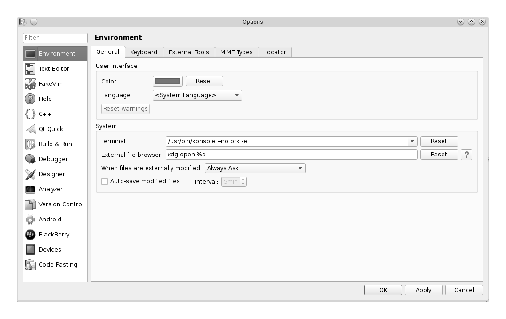
\includegraphics[width=0.7\textwidth]{img/ris_11_2}
\caption[Окно диалога настроек \Sys{Qt Creator}]{Окно диалога настроек \Sys{Qt Creator}}
\label{ch11:refDrawing1}
\end{center}
\end{figure}

Среди настроек редактора стоит отметить \index{Горячие клавиши!\Sys{Qt Creator}}настройки горячих клавиш. 
\Sys{Qt Creator} предоставляет множество комбинаций клавиш для выполнения различных действий. 
Приведем некоторые из них (см. табл.~\ref{ch11:refTable0}), которые
используются чаще всего.

{\noindent\small
\begin{longtable}{|p{0.18\textwidth}|p{0.74\textwidth}|}
\caption{Некоторые важные горячие клавиши \Sys{Qt Creator}} \label{ch11:refTable0}\\
\hline
\Emph{Комбинация клавиш}&\Emph{Описание}\\
\hline \hline
\endfirsthead
\multicolumn{2}{c}%
{{\tablename\ \thetable{} --- продолжение}} \\
\hline
\Emph{Комбинация клавиш}&\Emph{Описание}\\
\hline \hline
\endhead
\Sys{Esc} &
Выполняет переход к редактированию кода. Несколько последовательных нажатий этой клавиши переключают
пользователя в режим редактирования, закрывают панели вывода справки, отладки.\\\hline
\Sys{F4} &
Переключает редактор между файлом реализации (\Sys{.сpp}) и соответствующим заголовочным файлом (\Sys{.h}), которые
содержат объявления интерфейса и реализации класса в соотвенно.\\\hline
\Sys{F2} &
Выполняет переход к месту объявления переменной, функции, класса, на имени которых стоял курсор при
нажатии.\\\hline
\Sys{F1} &
Показывает справку для класса или метода \Sys{Qt}, на имени которого стоит курсор.\\\hline
\Sys{Ctrl+Shift+R} &
Переименование переменной, метода, класса, на имени которых стоит курсор. Имя будет изменено во всех
местах, где встречается его использование: не только в текущем файле, но и в других файлах проекта. При замене имени
будет учитываться область видимости имени, поэтому замена произойдет только в местах обращения к имени.
Именно этим это действие отличается от обычного поиска и замены текста.\\\hline
\Sys{Ctrl+Shift+U} &
Поиск всех мест обращения к переменной, методу, классу на имени которого стоит курсор.\\\hline
\Sys{Ctrl+K} &
Открывает поле быстрого поиска (Locator).\\\hline
\Sys{Alt+Enter} &
Позволяет открыть доступные дополнительные действия для переменной, метода, класса, оператора в позиции
курсора. Это дополнительные действия для рефакторинга (реорганизации и улучшения
существующего кода) могут содержать изменение порядка параметров, изменения в текущем фрагменте кода, добавление
фрагментов кода и т.д.\\\hline
\Sys{Ctrl+Space} &
Вызывает выпадающий список автозавершения код.\\\hline
\Sys{Ctrl+F} &
Поиск текста в текущем открытом файле.\\\hline
\Sys{Ctrl+Shift+F} &
Расширенный поиск текста в файле, проекте или группе проектов (доступны дополнительные
настройки).\\\hline
\end{longtable}
}

\subsection[Первый оконный проект]{Первый оконный проект}

Для \index{Создание!оконного проекта}создания простого оконного проекта выберите в главном меню 
\Sys{File->New File or Project...(Файл->Новый файл или проект...)} или нажмите 
\Sys{Ctrl+N}. На экране появится окно мастера новых файлов и проектов (см. рис.~\ref{ch11:refDrawing2}).

\begin{figure}[htb]
\begin{center}
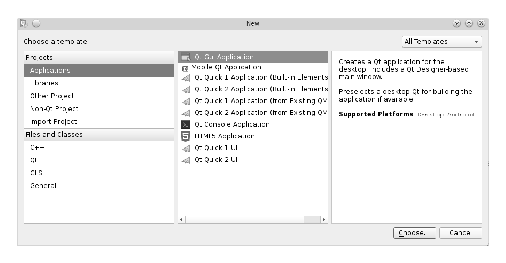
\includegraphics[width=0.7\textwidth]{img/ris_11_3}
\caption{Окно мастера новых файлов и проектов (шаг 1)}
\label{ch11:refDrawing2}
\end{center}
\end{figure}

Для создания нашего проекта выберем раздел \Sys{Applications(Приложения)} в списке
\Sys{Projects(Проекты)} и выберем \Sys{Qt Widgets Application} как тип проекта 
(приложение на \Sys{Qt} с использованием виджетов). Нажмем кнопку \Sys{Choose...(Выбрать...)}.

Далее нам необходимо ввести имя проекта в поле ввода \Sys{Name} (например
\Sys{FirstGuiProject}). Поле ввода \Sys{Create in} содержит путь, где
будет создан каталог с новым проектом. Флажок 
\Sys{Use as default project location}(\Sys{Использовать как место по умолчанию для размещения проектов})
означает, что путь расположения проекта сохраняется и для последующих новых проектов (рис.~\ref{ch11:refDrawing3})

\begin{figure}[htb]
\begin{center}
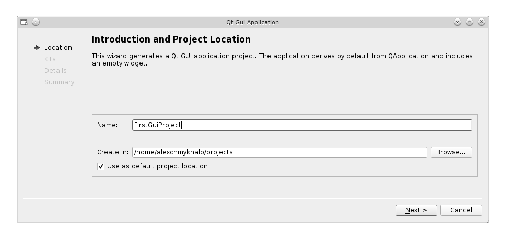
\includegraphics[width=0.7\textwidth]{img/ris_11_4}
\caption{Окно мастера новых файлов и проектов (шаг 2)}
\label{ch11:refDrawing3}
\end{center}
\end{figure}

Во время следующего шага (рис.~\ref{ch11:refDrawing4}) необходимо указать
комплект, с помощью которого среда будет строить новый проект. Оставим выбор
инструментария по умолчанию и нажмем кнопку \Sys{Next (Далее)}.

\begin{figure}[htb]
\begin{center}
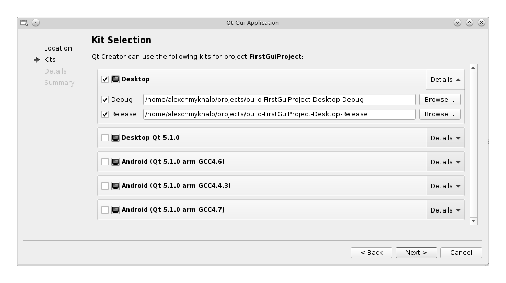
\includegraphics[width=0.7\textwidth]{img/ris_11_5}
\caption{Окно мастера новых файлов и проектов (шаг 3)}
\label{ch11:refDrawing4}
\end{center}
\end{figure}

Следующее окно мастера (см. рис.~\ref{ch11:refDrawing5}) информирует о классах, которые
будут сгенерированы автоматически для нового проекта. Для главного окна программы будет сгенерирован класс
\Sys{MainWindow} (поле \Sys{Class name}), который будет
унаследован от класса \Sys{QMainWindow} (поле {\Sys{Base class}).
Класс \index{Класс!\Sys{QMainWindow}}\Sys{QMainWindow} обладает особенностями, характерными 
для главного окна программы, такими как главное меню, панель
инструментов и т.п. Для кода класса \Sys{MainWindow} мастер создаст заголовочный файл --- 
\Sys{mainwindow.h} (поле \Sys{Header file}) и файл реализации --- 
\Sys{mainwndow.cpp} (поле \Sys{Source file}), а также добавит их
в проект.

Флажок \Sys{Generate form} указывает на необходимость сгенерировать и добавить
к проекту файл формы для главного окна. 

\begin{figure}[htb]
\begin{center}
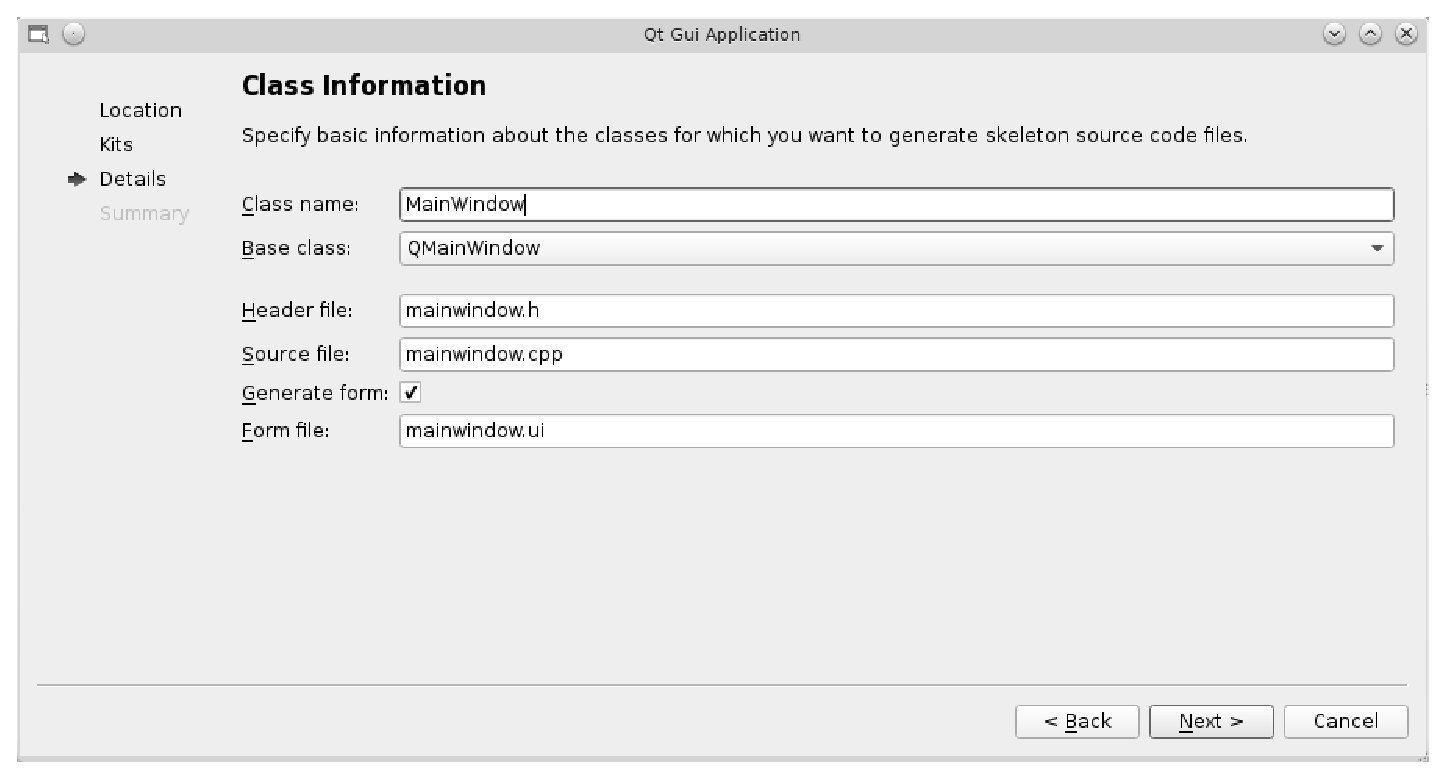
\includegraphics[width=0.7\textwidth]{img/ris_11_6}
\caption{Окно мастера новых файлов и проектов (шаг 4)}
\label{ch11:refDrawing5}
\end{center}
\end{figure}

\begin{figure}[htb]
\begin{center}
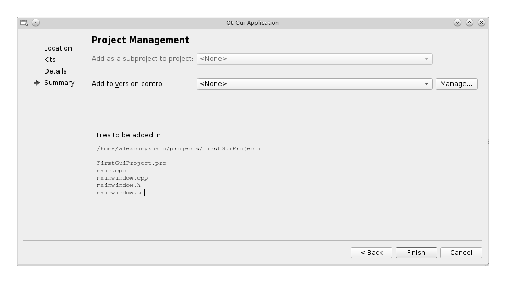
\includegraphics[width=0.7\textwidth]{img/ris_11_7}
\caption{Окно мастера новых файлов и проектов (шаг 5)}
\label{ch11:refDrawing6}
\end{center}
\end{figure}

В завершающем окне мастера (см. рис.~\ref{ch11:refDrawing6}) нажмите
\Sys{Finish (Завершить)}.

Файлы \index{Файл!формы}формы позволяют редактировать вид окна с помощью 
визуального редактора интерфейса --- \index{Инструменты Qt!Qt Designer}\Sys{Qt Designer}. 
Оболочка \Sys{Qt Creator} также дает
возможность редактировать файлы формы. Файлы формы главного окна будет сгенерирован 
автоматически --- \Sys{mainwindow.ui} (поле \Sys{Form file}).

После завершения работы мастера проект откроется в окне оболочки \Sys{Qt Creator}.
В левой части окна теперь можно исследовать структуру проекта, который состоит из всех файлов, входящих в
проект и были сгенерированы мастером. Для компиляции и запуска проекта нажмите кнопку запуска программы или комбинацию
клавиш \Sys{Ctrl R}. После запуска появится пустое окно --- главное окно нашей программы. Вот
таким образом выглядит создание простого оконного проекта. Все файлы проекта были сгенерированы
мастером, который используют обычно для удобства и чтобы ускорить работу. Конечно, есть и другой путь --- можно создать
каждый из файлов отдельно и, без каких-либо трудностей, добавить к проекту. Мы подробно рассмотрим как это делать, для
того, чтобы исследовать основные составляющие проекта \Sys{Qt} и понять как происходит его компиляция.

\section[Задачи для самостоятельного решения]{Задачи для самостоятельного решения}
\begin{enumerate}
\item Повторите описанные шаги для создания собственного проекта. Назовите проект \Sys{MyGuiProject}. Класс
главного окна программы назовите \Sys{MyMainWindow}. Просмотрите структуру проекта. Скомпилируйте и запустите проект
на выполнение. 
\item Попробуйте использовать любую из горячих клавиш, описанных в таблице <<Некоторые
важные горячие клавиши>>. 
\item Используйте документацию \Sys{Qt} и найдите описание для классов \Sys{QMainWindow} и \Sys{QApplication}. 
\end{enumerate}
